\section{Theorie}
\subsection{Semiklassische Herleitung}
Ein Hg-Atom welches ein Photon absorbiert kann als ein gedämpfter oszillierender Dipol beschrieben werden. Die Dipolachse ist dabei parallel zur Polarisation des absorbierten Photons. Zur Bestimmung der gesamt Intensität eines einzelnen angeregten Atoms muss über alle Zeiten integriert werden wodurch sich folgende Gleichung ergibt.
\begin{equation}
	I=C\cdot \int_{0}^{\infty}sin(\phi)^2e^{-\frac{t}{\tau}}dt
\end{equation}
Hierbei ist zu erkennen das die Strahlungscharakteristik proportional zu $sin(\phi)^2$ ist, wobei $\phi$ der Winkel zischen Dipolachse und Beobachtungsrichtung ist. Der Faktor $e^{-\frac{t}{\tau}}$ beschreibt die Dämpfung.\par
Wenn nun ein Magnetfeld angelegt wird und dieses senkrecht auf der Oszillation-Achse liegt so wird ein Drehmoment auf den Dipol ausgeübt. Dieses führt zur Präzision des Dipols und des magnetischen Moments welches hier als starr zusammenhängend betrachtet wird. Für das magnetische Moment $\mu$ eines Niveaus mit Drehimpulsquantenzahl J gilt
im schwachen Feld folgende Bewegungsgleichung:
\begin{equation}
\frac{d\vec{\mu}}{dt}=\frac{\omega_L}{B}\vec{\mu}\times\vec{B}
\label{Präzesion}
\end{equation}
hierbei ist $\omega_L$ die Larmorfrequenz mit:
\begin{equation}
	\omega_L=g_J\frac{\mu_B}{\hbar}B
\end{equation}
Grafisch wird die Bewegung in Abbildung \ref{Präzesionsbild} dargestellt.
\begin{figure}[ht]
	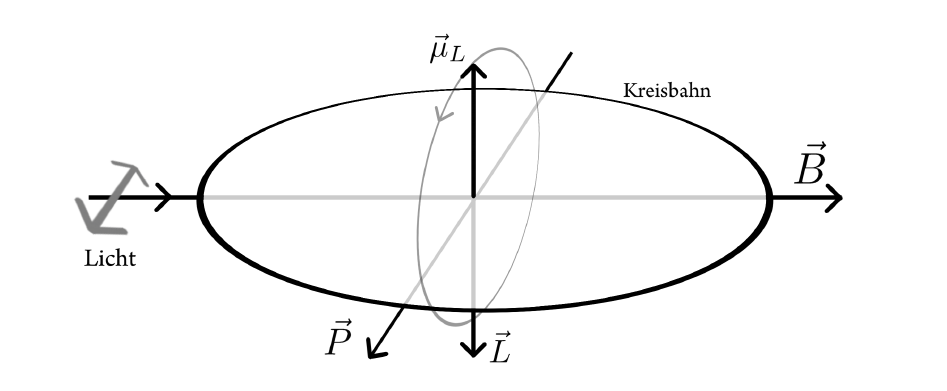
\includegraphics[scale=0.8]{Bild/TestP}
	\centering
	\caption{2: Darstellung der Präzessionsbewegung eines Elektrons mit Dipolmoment $\vec{P}$, Drehimpuls $\vec{L}$ und magnetischem Moment $\mu_L$ bei angelegtem Magnetfeld der Flussdichte $B$.}
	\label{Präzesionsbild}
\end{figure}\\
Sind Polarisation (und somit auch Dipolachse) zum Zeitpunkt der Absorption parallel zur Beobachtungsebene gilt $\theta(t)=\omega_Lt$ mit $\theta(t=0)=0$. Das bedeutet für die Intensität:
\begin{equation}
	I=C\cdot \int_{0}^{\infty}\sin(\phi)^2e^{-\frac{t}{\tau}}dt=\frac{C\tau}{2}\left(\frac{(2\omega_L\tau)^2}{1+(2\omega_L\tau)^2}\right)
	\label{GLStuff}
\end{equation}
Ist die Beobachtungsrichtung zum Zeitpunkt der Absorption senkrecht zur Polarisationsrichtung gilt: $\theta(t)=\omega_Lt+\frac{\pi}{2}$ mit $\theta(t=0)=\frac{\pi}{2}$. Die Intensität lässt sich ähnlich wie in Gleichung \ref{GLStuff} beschreiben:
\begin{equation}
I=C\cdot \int_{0}^{\infty}\cos(\phi)^2e^{-\frac{t}{\tau}}dt=\frac{C\tau}{2}\left(2-\frac{(2\omega_L\tau)^2}{1+(2\omega_L\tau)^2}\right)
\label{GLStuff2}
\end{equation}
Die Gleichung \ref{GLStuff} entspricht einer inversen Lorenz-kurve und Gleichung \ref{GLStuff2} einer normalen. Die Lebensdauer $\tau$ dieser Kurven kann über die Breite der Funktion auf halber Höhe (\textit{eng: Full width at half maximum (FWHM)}) bestimmt werden (siehe Abb.\ref{Lorenzbild}). Hierfür gilt:
\begin{equation}
	\tau=\frac{\hbar}{g_J\mu_BB_{FW}}
\end{equation}
\begin{figure}
	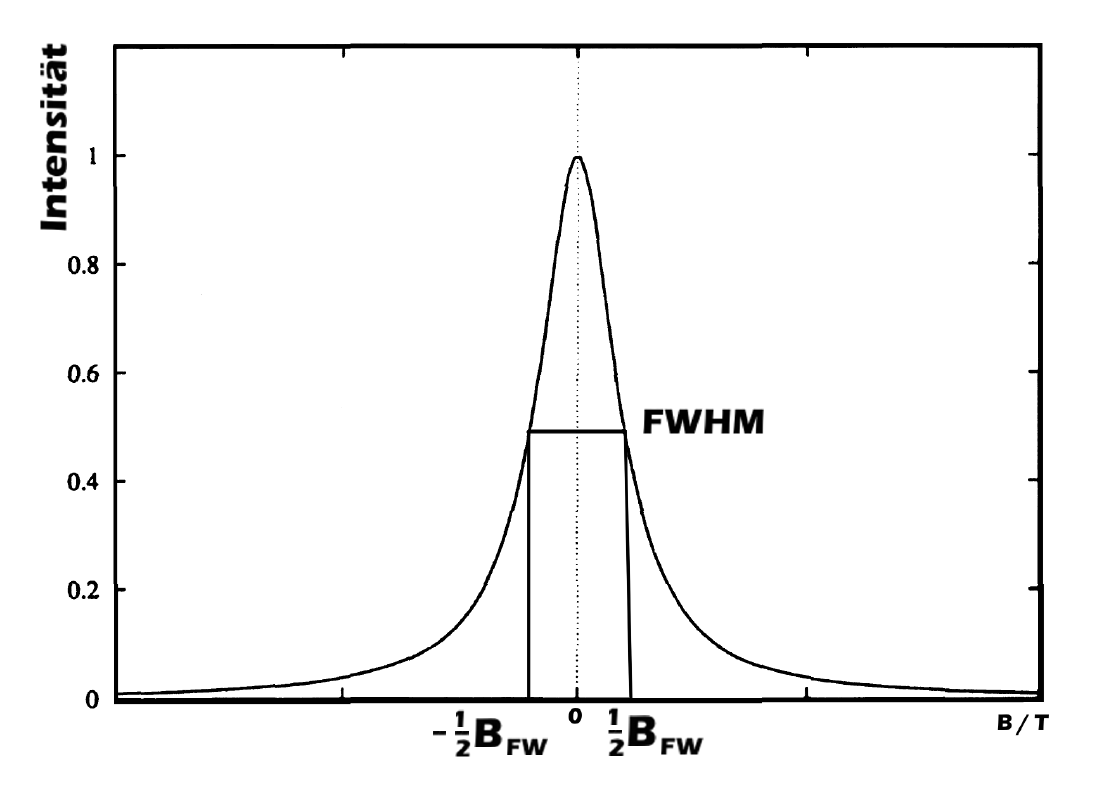
\includegraphics[scale=0.7]{Bild/Lorenz}
	\centering
	\caption{Lorentzkurve mit sichtbare Intensität in Beobachtungsrichtung $0^\circ$ mit FWHM eingezeichnet.}
	\label{Lorenzbild}
\end{figure}
\subsection{Quantenmechanische Erklärung}
In der Quantenmechanik wird das Phänomen der Resonanzfluoreszenz durch Interferenz sich überlagernder Zustände beschrieben. Zustände unterschiedlicher magnetischer Quantenzahl $m_j$ sind im Allgemeinen erst einmal energetisch gleich, “entartet“. Die Entartung kann aber durch Anlegen eines Magnetfeldes aufgehoben werden (Zeeman-Effekt). In Spezialfällen verursacht die Kreuzung zweier Niveaus von Zuständen verschiedener Gesamtdrehimpulse, bei bestimmten Magnetfeldstärken, eine weitere Entartung. 
\begin{figure}[ht]
	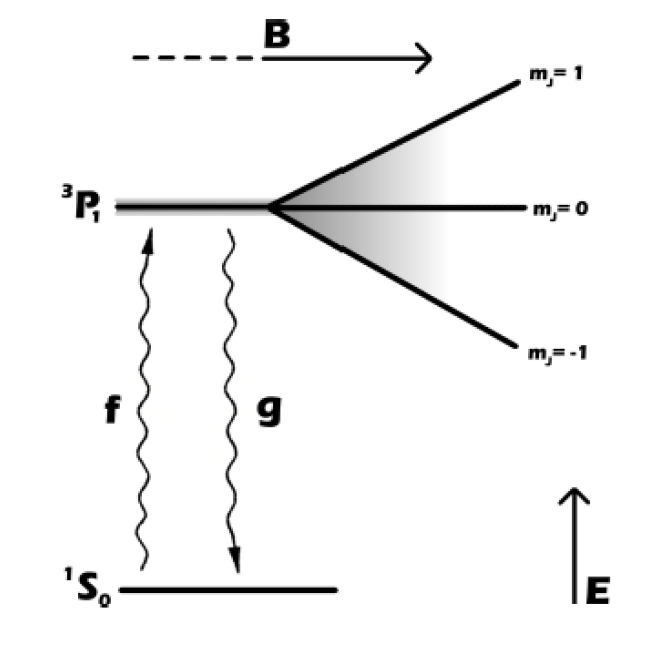
\includegraphics[scale=0.6]{Bild/Zeeman}
	\centering
	\caption{Aufspaltung der Energieniveaus durch $m_j$ in einem Magnetfeld.}
\end{figure}
Liegt keine Energieaufspaltung vor werden die Niveaus kohärent angeregt werden und bei Abregung kommt es zur Interferenz mehrerer Zustände des selben Atoms. Damit gilt:
\begin{equation}
	I\propto(A_1+A_2)^2
\end{equation}
Bei einer Aufspaltung der Niveaus können die Niveaus getrennt angeregt und abgeregt werden. Für die gesamt Intensität gilt dann:
\begin{equation}
I\propto A_1^2+A_2^2
\end{equation}